\documentclass[11pt,a4paper]{article}
\usepackage[utf8]{inputenc}
\usepackage[german]{babel}
\usepackage[T1]{fontenc}
\usepackage{amsmath}
\usepackage{amsfonts}
\usepackage{amssymb}
\usepackage{graphicx}
\usepackage{pstricks}
\usepackage{float}
\usepackage{tikz}
\usepackage{pgfplots}
\usepackage{asymptote}
\usepackage{mathptmx}
\usepackage{caption}
\usepackage[left=2cm, right=2cm, top=2cm,bottom=2cm]{geometry}
\usepackage[colorlinks=true, urlcolor=blue, linkcolor=blue]{hyperref}
\title{Wellennachweis - Abtriebswelle}
\author{Quentin Huss, Nadine Schulz}
\date{21.06.2023}
\begin{document}
\maketitle

\section{Darstellung der Welle}
\begin{figure}[!h]
\centering
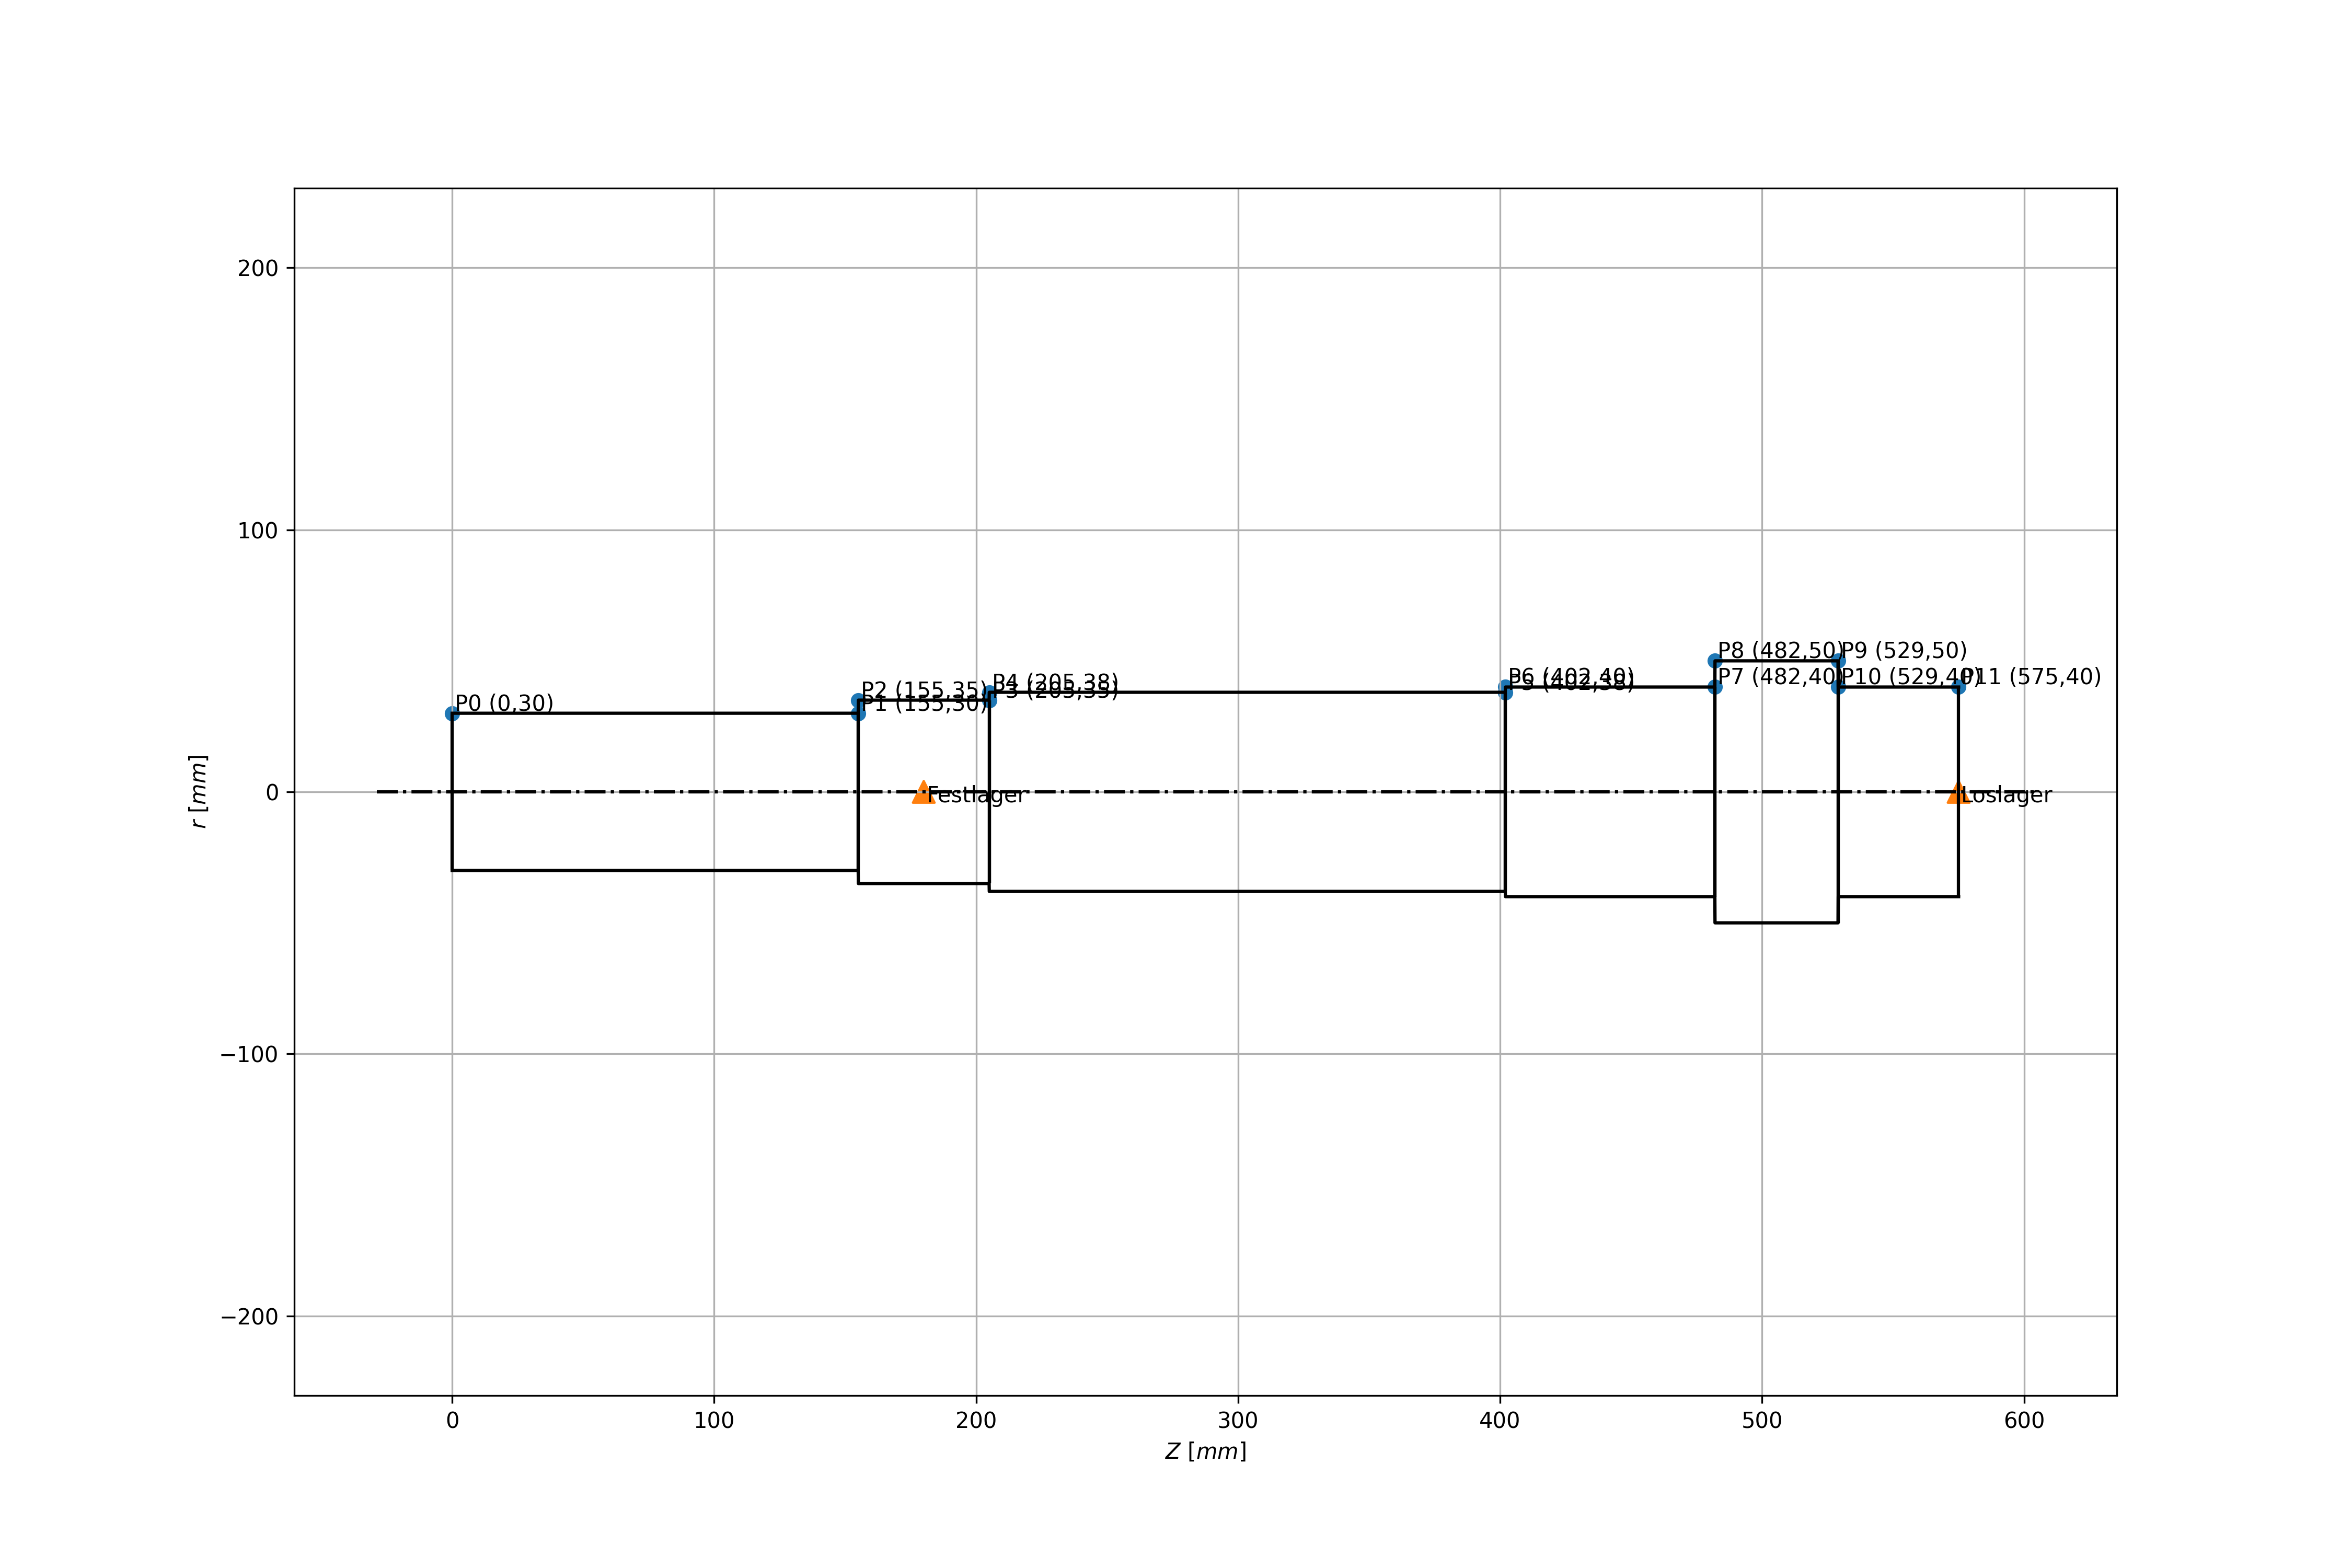
\includegraphics[scale=0.5]{AbtriebswelleWELLE.png}
\end{figure}

\pagebreak

\begin{figure}[!ht]
\section{Plots}
\centering
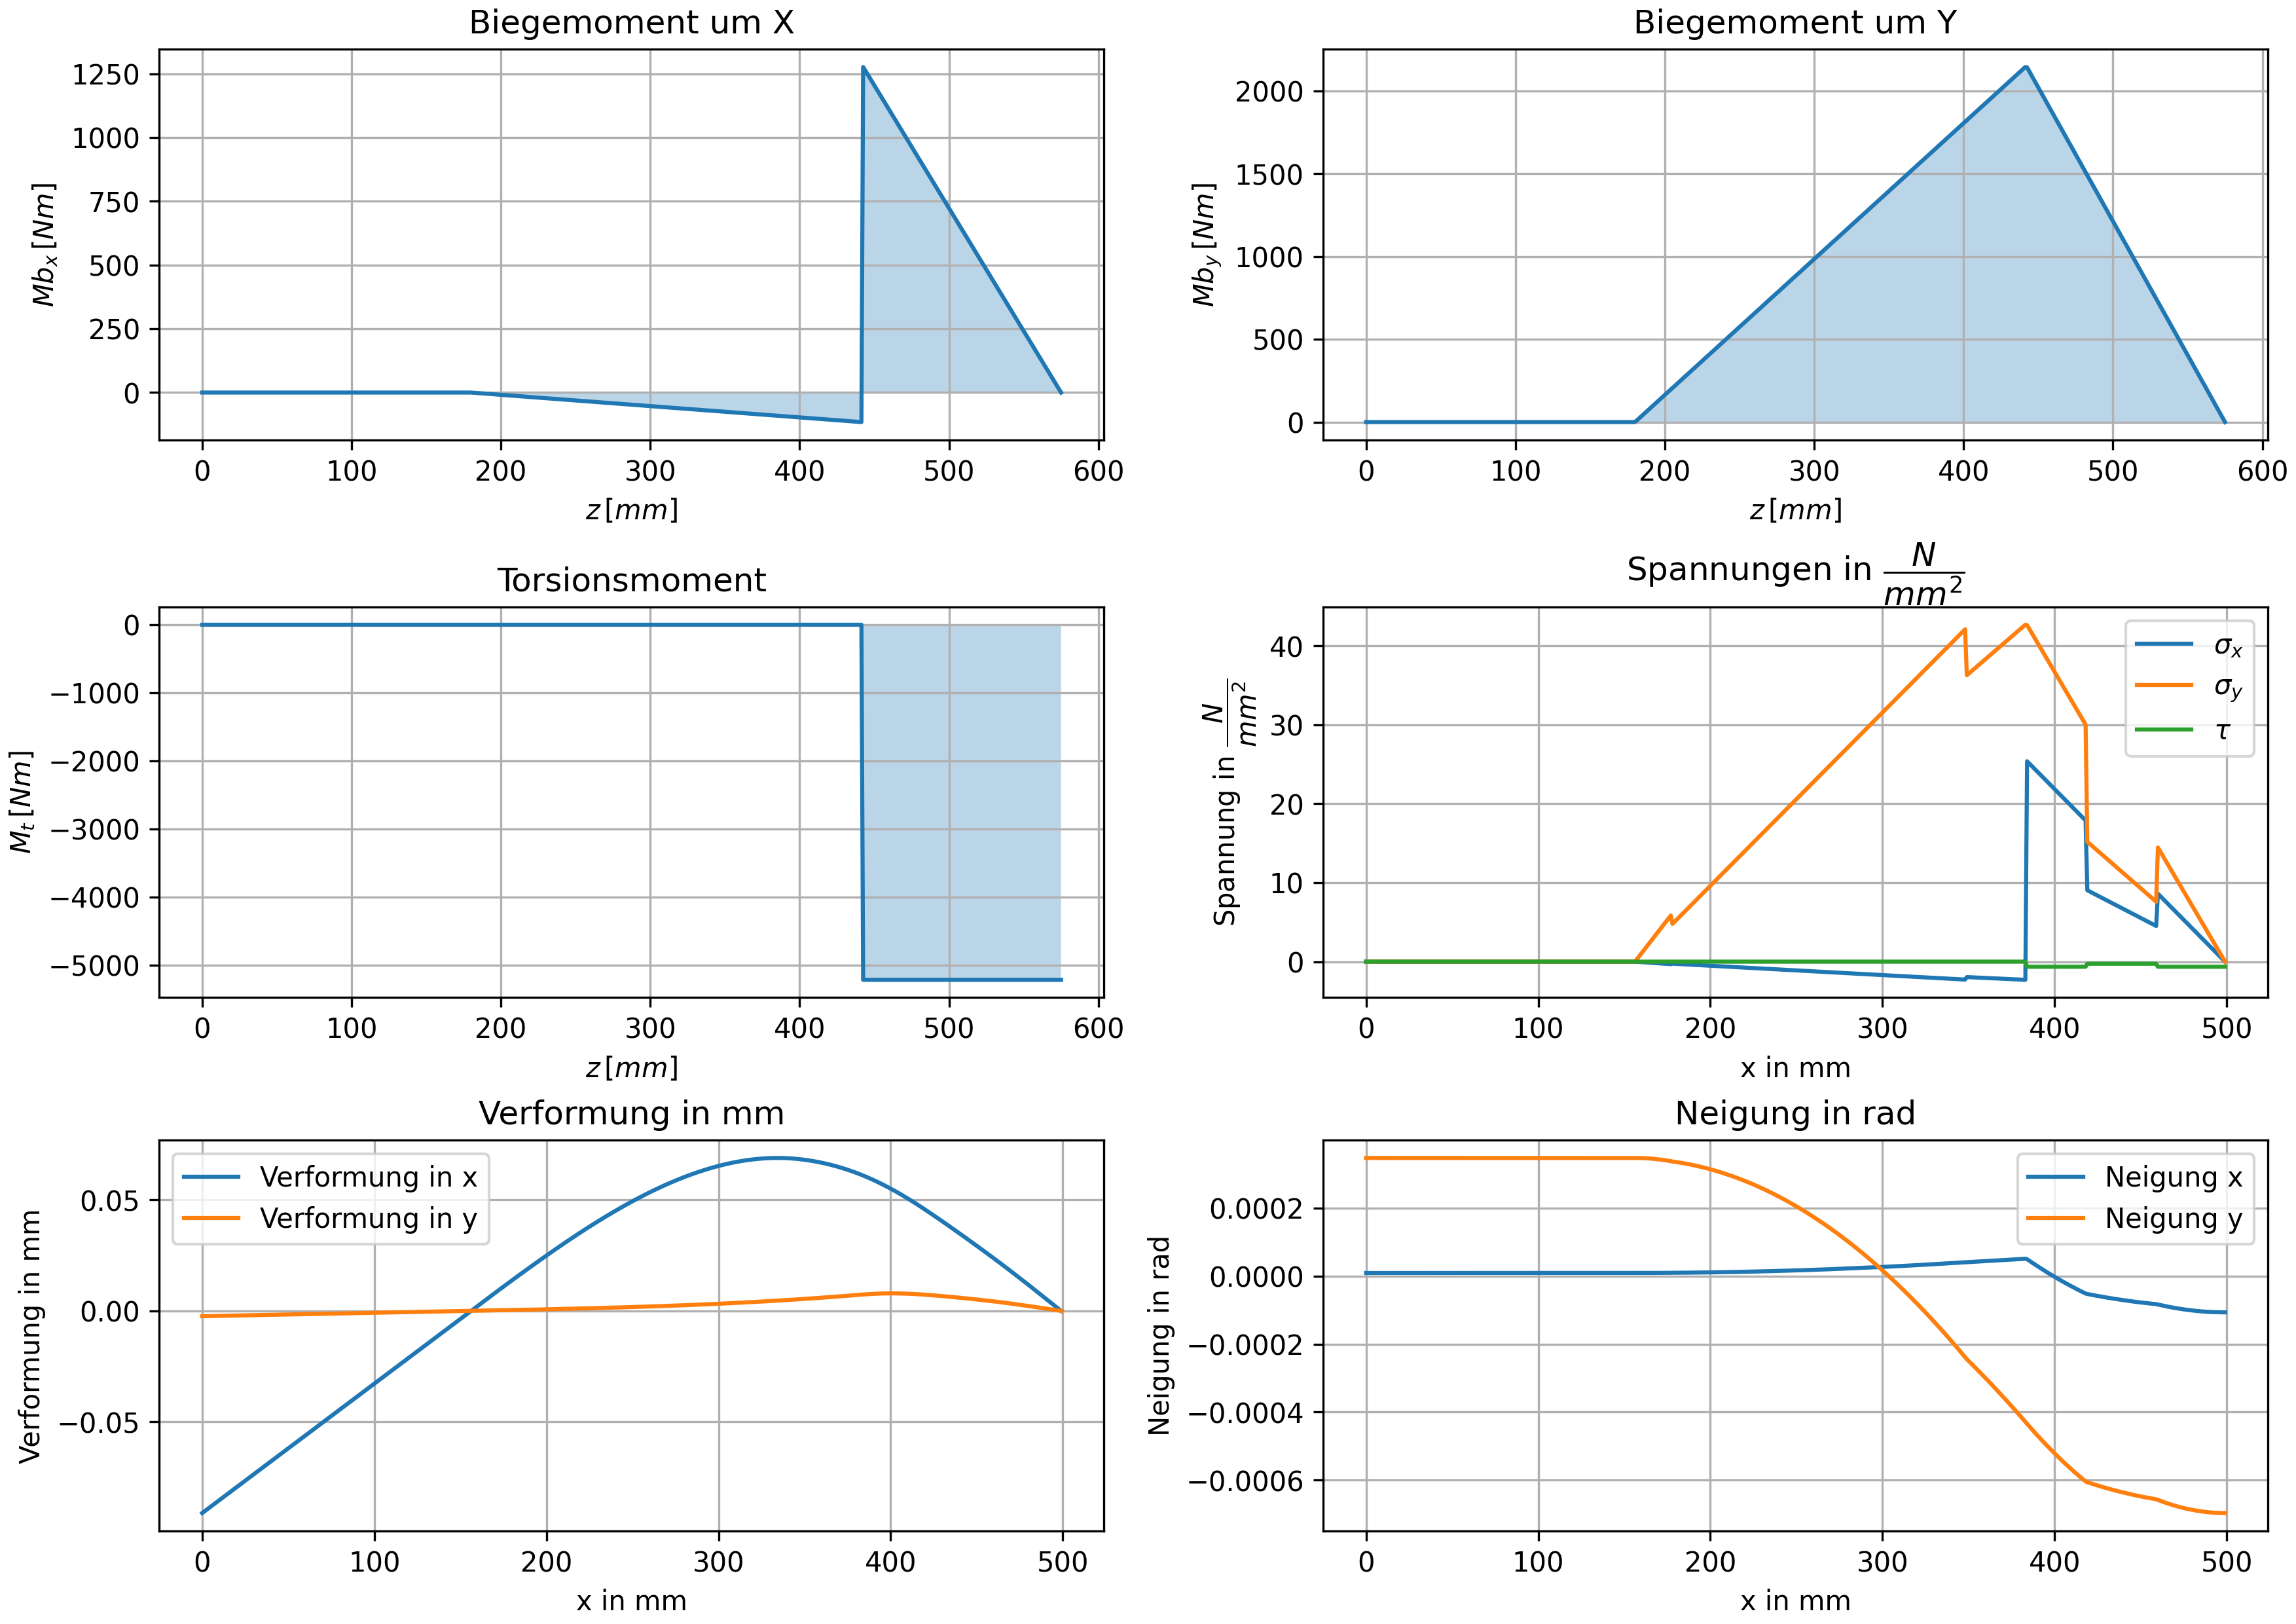
\includegraphics[scale=0.5]{Abtriebswelleplot.png}
\end{figure}



\section{Verformung und Neigung}

\begin{center}
\begin{tabular}{|lll|}
maximale Verformung in x: & 0.0688736170697904& $\mu m$ \\
Verformungsgradient in x: & 0.1743635875184568& $\dfrac{mm}{m}$ \\
maximale Verformung in y: & 0.0078775679143873& $\mu m$ \\
Verformungsgradient in y: &0.0199432099098414& $\dfrac{mm}{m}$ \\
maximale Verformung addiert: & 0.0910852735731127& $\mu m$ \\
Verformungsgradient addiert: &0.2305956292990197& $\dfrac{mm}{m}$ \\
\hline 
Neigung im Festlager x: &9.168591381543824e-06& rad \\
Neigung im Festlager y: &0.0003474993853309& rad \\
Neigung im Loslager x: &-0.0001065510646933& rad \\
Neigung im Loslager y: &-0.0006968473930314& rad \\
\end{tabular}
\end{center}


\section*{Absatz an Stelle 155 mm}

\subsection*{Geometrie}

\begin{center}
\begin{tabular}{|ll|}
großer Durchmesser & $D =70.0\ mm$ \\
kleiner Durchmesser & $d =60.0\ mm$ \\
Radius & $r =5\ mm$ \\
Absatzsprung & $t =5.0\ mm$
\end{tabular}
\end{center}

\section*{Absatz an Stelle 402 mm}

\subsection*{Geometrie}

\begin{center}
\begin{tabular}{|ll|}
großer Durchmesser & $D =80.0\ mm$ \\
kleiner Durchmesser & $d =76.0\ mm$ \\
Radius & $r =5\ mm$ \\
Absatzsprung & $t =2.0\ mm$
\end{tabular}
\end{center}

\section*{Absatz an Stelle 482 mm}

\subsection*{Geometrie}

\begin{center}
\begin{tabular}{|ll|}
großer Durchmesser & $D =100.0\ mm$ \\
kleiner Durchmesser & $d =80.0\ mm$ \\
Radius & $r =1\ mm$ \\
Absatzsprung & $t =10.0\ mm$
\end{tabular}
\end{center}
\end{document}